\subsection{Kegelschnitte}

\subsubsection{Allgemeine Form}

\[
    A x^2 + B y^2 + C x + D y + E = \sigma
\]

\subsubsection{Kreis}

\[
    A = B
\]

\begin{figure}[H]
    \centering
    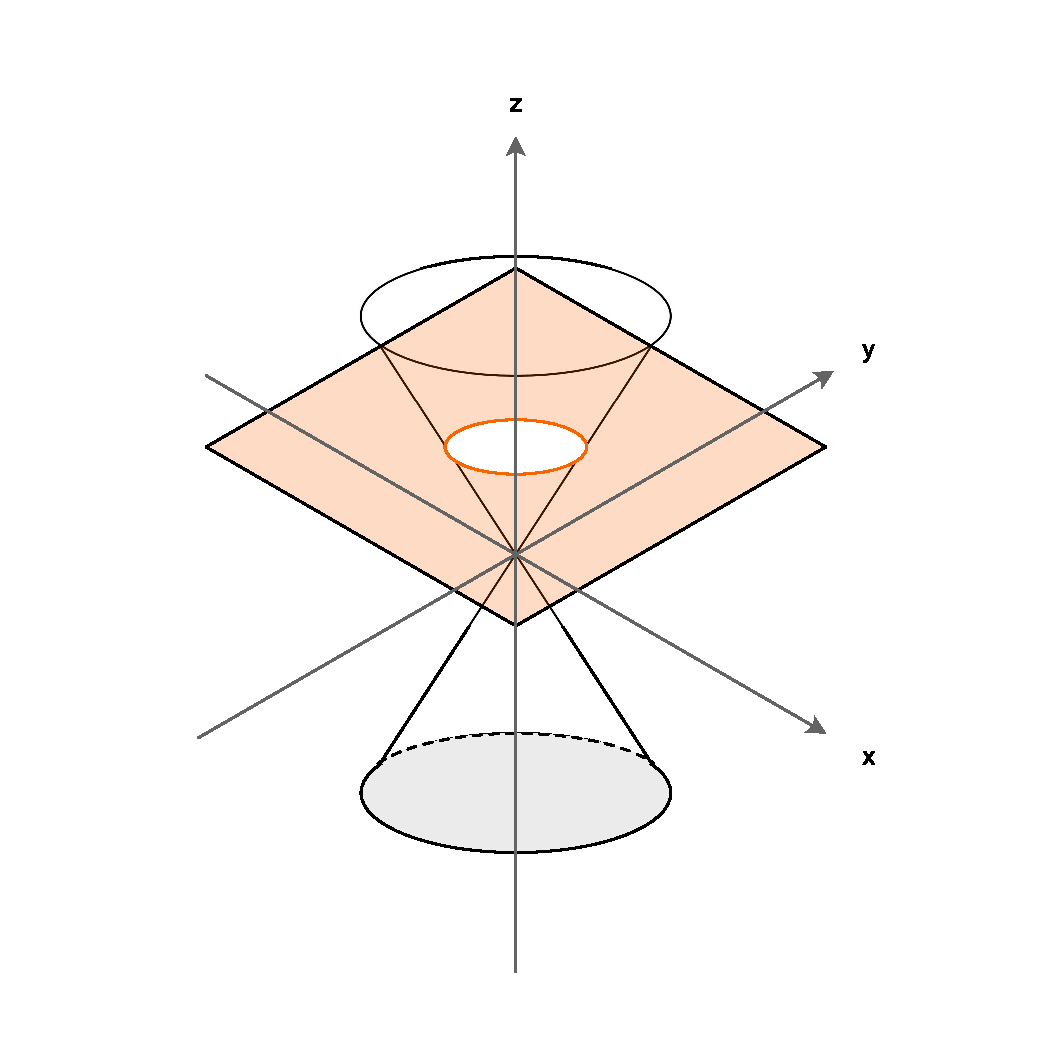
\includegraphics[width=8cm]{grafiken/kegelschnitte/kreis}
    \begin{tikzpicture}
        \begin{axis}[
                defaultnonumbers,
                xmin=-1.2, xmax=1.2,
                ymin=-1.2, ymax=1.2,
                width=8cm
            ]
            \draw (0,0) circle [radius=1];
        \end{axis}
    \end{tikzpicture}
    \caption{Kegelschnitt: Kreis}
\end{figure}

\paragraph{Einheitskreis}

\[
    A = B = 1 \quad E = -1 \quad x^2 + y^2 = 1  
\]

\paragraph{Hauptform vom Kreis}

\[
    {(x - x_0)}^2 + {(y - y_0)}^2 = r^2
\]


\subsubsection{Ellipse}

\[
    A \cdot B > 0, A \neq B  
\]

\begin{figure}[H]
    \centering
    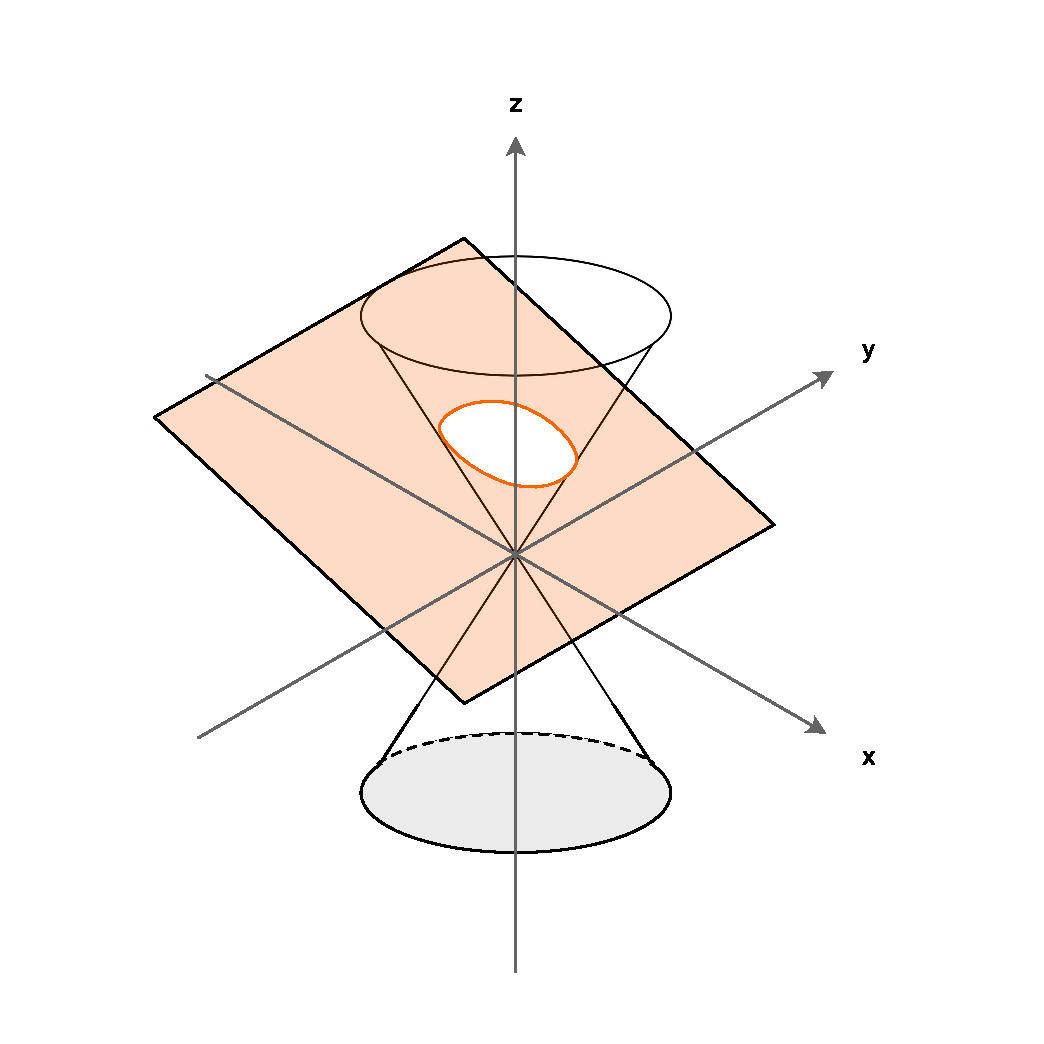
\includegraphics[width=8cm]{grafiken/kegelschnitte/ellipse}
    \begin{tikzpicture}
        \begin{axis}[
                defaultnonumbers,
                xmin=-2.2, xmax=2.2,
                ymin=-1.2, ymax=1.2,
                width=8cm
            ]
            \draw (0,0) ellipse (2 and 1);
        \end{axis}
    \end{tikzpicture}
    \caption{Kegelschnitt: Ellipse}
\end{figure}

% \includegraphics{grafiken/Kegelschnitt_Ellipse}

\subsubsection{Hyperbel}

\[
    A \cdot B < 0, a \neq B
\]

\begin{figure}[H]
    \centering
    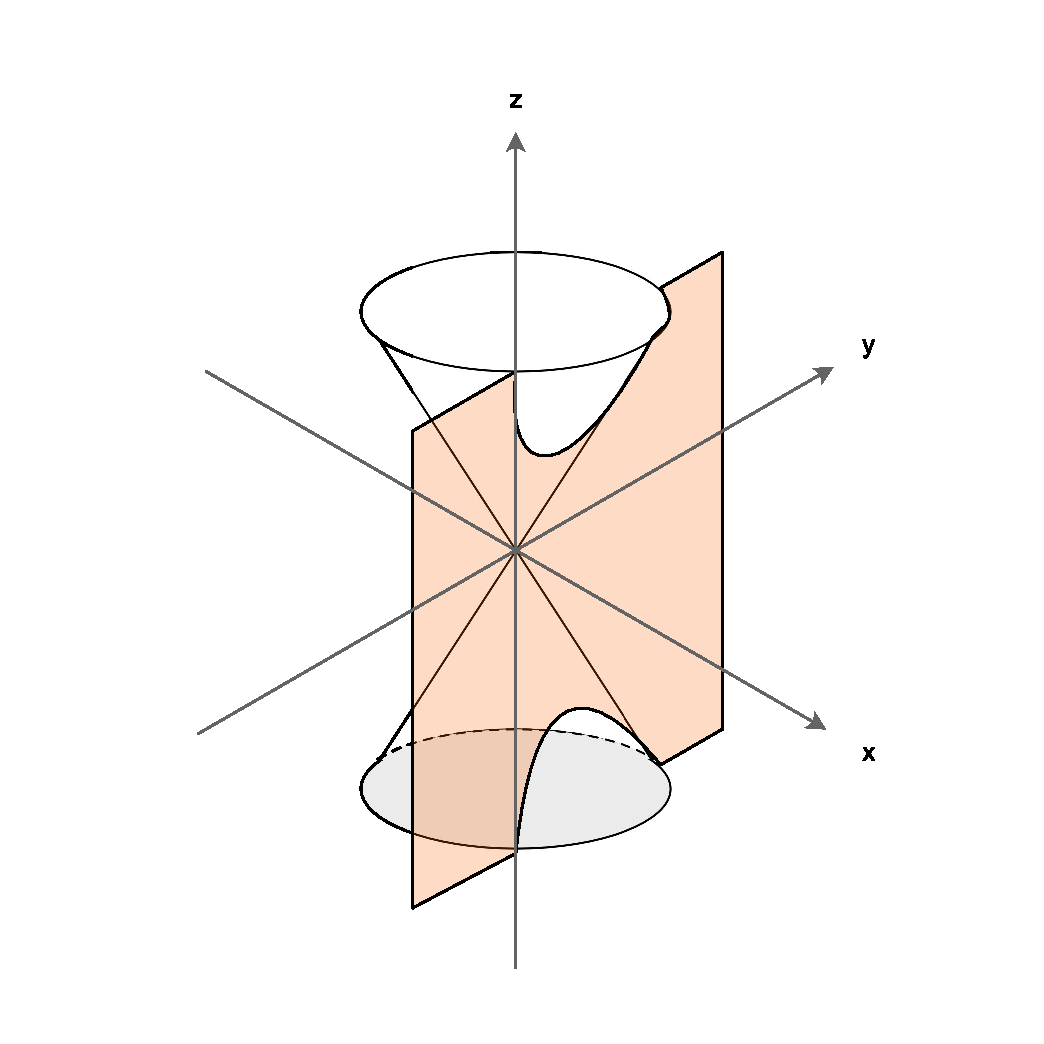
\includegraphics[width=8cm]{grafiken/kegelschnitte/hyperbel}
    \begin{tikzpicture}
        \begin{axis}[
                defaultnonumbers,
                xmin=-2.2, xmax=2.2,
                ymin=-2.2, ymax=2.2,
                width=8cm
            ]
            \addplot [domain=-2:2] ({cosh(x)}, {sinh(x)});
            \addplot [domain=-2:2] ({-cosh(x)}, {sinh(x)});
        \end{axis}
    \end{tikzpicture}
    \caption{Kegelschnitt: Hyperbel}
\end{figure}

\subsubsection{Parabel}

\[
    (A = 0 \wedge B \neq 0) \vee (A \neq 0 \wedge B = 0)    
\]

\begin{figure}[H]
    \centering
    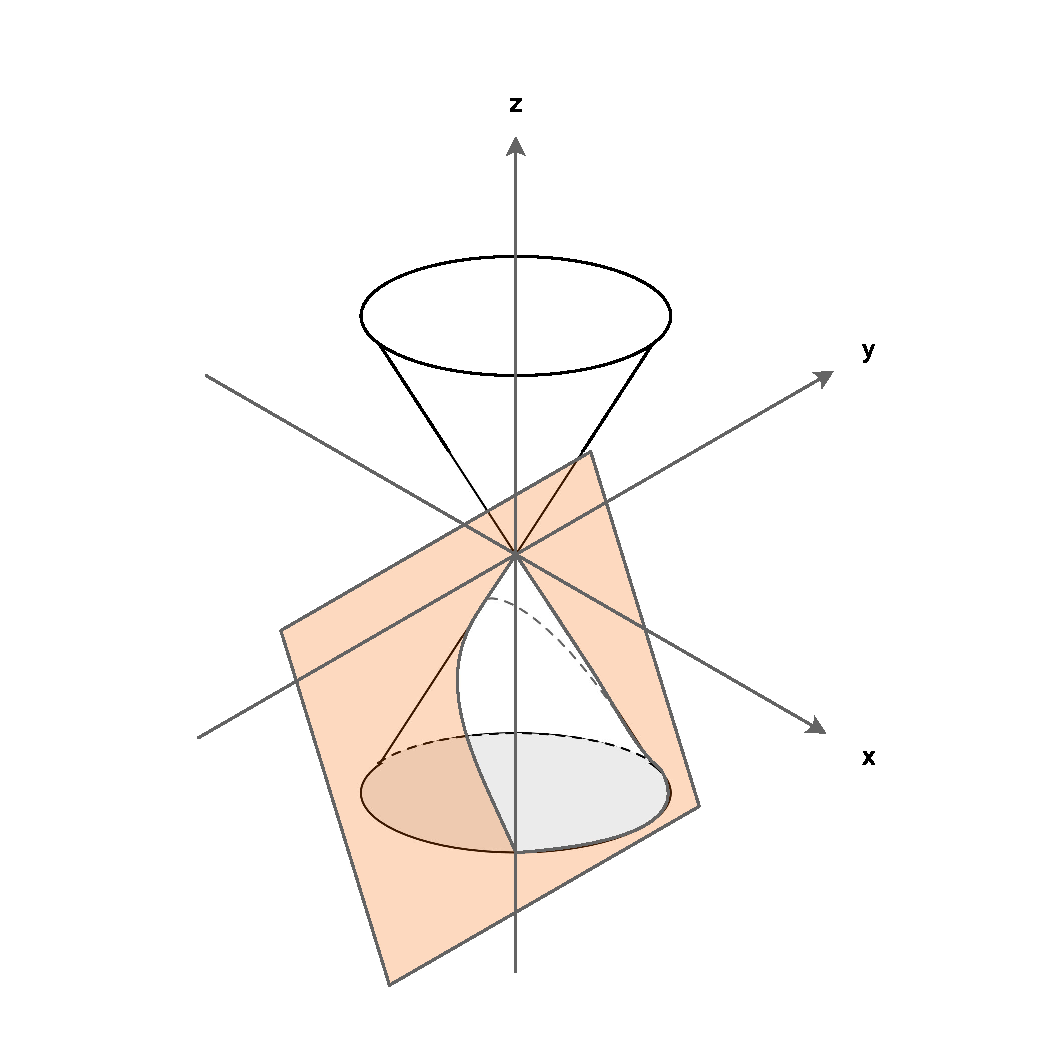
\includegraphics[width=8cm]{grafiken/kegelschnitte/parabel}
    \begin{tikzpicture}
        \begin{axis}[
                defaultnonumbers,
                xmin=-2.2, xmax=2.2,
                ymin=-2.2, ymax=2.2,
                width=8cm
            ]
            \addplot [domain=-2:2] {x^2};
        \end{axis}
    \end{tikzpicture}
    \caption{Kegelschnitt: Parabel}
\end{figure}
